\chapter{Hardware}

Como ya se ha comentado previamente, el \textbf{hardware} es todo lo que forma parte del ordenador, que \textbf{puede ser tocado físicamente}. Dentro de un ordenador vamos a poder diferenciar distintos componentes que cumplirán una función distinta que detallaremos más adelante.

Es posible que ya conozcamos alguno de estos componentes, pero debemos conocer el origen y cómo surge la arquitectura de los ordenadores modernos.


\section{Arquitectura Von Neumann}

Las primeras computadoras electromecánicas eran diseñadas para un único propósito, estaban “diseñadas” para realizar una tarea. Un caso conocido puede ser \href{https://es.wikipedia.org/wiki/Bombe}{\textbf{Bombe}}, una máquina electromecánica capaz de descifrar los sistemas criptográficos nazis de Enigma. \movie{https://www.imdb.com/title/tt2084970/}{The Imitation Game}

Algunas se podían “reprogramar”, pero a base de recablear distintos componentes tras un estudio de lo que se quería realizar. Podía tomar hasta tres semanas preparar un programa de ENIAC y conseguir que funcionara.

El concepto de máquinas de computación universal y el uso de programa almacenado ya existía a nivel teórico desde mediados de la década de 1930 (escrito por \href{https://es.wikipedia.org/wiki/Alan_Turing}{Alan Turing}).

El matemático y físico \href{https://es.wikipedia.org/wiki/John_von_Neumann}{John von Neumann}, junto con otros compañeros, \textbf{describe en 1945 un diseño para una arquitectura de computadoras} en el que se describren los siguientes componentes que se interrelacionan entre sí a través del bus del sistema que actúa como canal de comunicación entre ellos:

\vspace{-10pt}
\begin{center}
    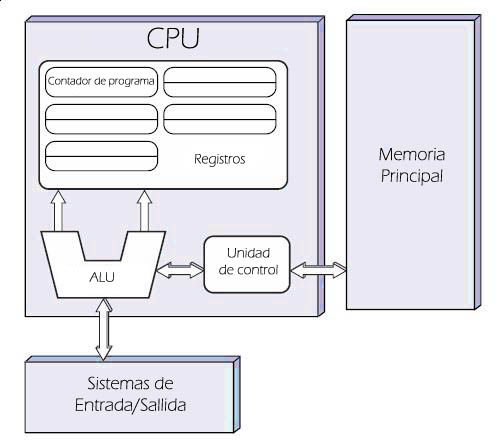
\includegraphics[width=0.5\linewidth]{vonneumann.jpg}
    \captionof{figure}{Arquitectura Von Neumann. Fuente: \href{https://es.wikipedia.org/wiki/Arquitectura_de_Von_Neumann}{wikipedia}}
\end{center}

\begin{itemize}
    \item \textbf{Unidad Central de Proceso} (\textbf{CPU}, por sus iniciales en inglés), que a su vez, contiene:
    \begin{itemize}
        \item \textbf{Unidad Aritmético Lógica} (\textbf{ALU} en inglés): Es un circuito digital que realiza operaciones aritméticas (suma, resta, multiplicaciones,...) y operaciones lógicas (AND, OR, X-OR,...) entre los valores de los argumentos (uno o dos).
        \item \textbf{Registros del procesador}: Memoria de alta velocidad y poca capacidad integrada en la CPU para almacenar datos utilizados durante la ejecución de un programa:
        \begin{itemize}
            \item Contador de programa
            \item Acumulador
            \item Registro de instrucciones
        \end{itemize}
        \item \textbf{Unidad de control}: Su función es buscar las instrucciones en la memoria principal, decodificarlas y ejecutarlas, empleando para ello la unidad de proceso.
    \end{itemize}
    \item La \textbf{memoria principal}: Sistema donde se almacenan las instrucciones y los datos del programa que se está ejecutando en ese instante, dividida en celdas que se identifican por medio de una única dirección.
    \item Los \textbf{sistemas de Entrada/Salida}: Realizan la transferencia de información entre periféricos de entrada y/o salida para extender las capacidades del equipo.
\end{itemize}


Hoy en día, los ordenadores han evolucionado, pero la arquitectura sigue siendo la misma, aunque más compleja.

\infobox{\textbf{Podemos ver una simulación de la Arquitectura Von Neumann \href{https://lab.xitrus.es/VonNeumann/}{aquí}}}


\section{Componentes básicos}

Un ordenador moderno se puede distinguir de distintos componentes, los cuales cumplen una función específica. Así mismo, también pueden contar con subcomponentes integrados que son necesarios para cumplir su cometido final.

A continuación se van a detallar los componentes necesarios de un ordenador moderno.

%\begin{itemize}
%    \item CPU / procesador
%    \item Placa base
%    \item Memoria
%    \item Tarjetas gráficas
%    \item Unidades de almacenamiento
%    \item Fuente de alimentación
%    \item Unidades de entrada
%    \item Unidades de salida
%    \item Unidades de entrada/salida
%    \item Caja del ordenador
%\end{itemize}

\subsection{Placa base}

La placa base (conocida en inglés como \textit{motherboard}) es una tarjeta de circuito impreso que tiene elementos electrónicos (resistencias, condensadores, reguladoresm ...)  a la que se conectan el resto de componentes que forman el ordenador. Es por eso que se puede considerar como la parte fundamental a la hora de montar un ordenador, ya que sin ella, el resto de componentes no se podrán comunicar entre sí.


\subsubsection{Formatos de placa base}
Las placas base deben tener un tamaño compatible con las cajas en las que van a ir montadas, y es por eso que hay distintos tamaños estandarizados. Cada uno de estos tamaños determinan dónde van a ir montados algunos de los componentes y conectores, así como los agujeros donde irán los tornillos de sujeción a la caja.

Si queremos profundizar más en los distintos formatos, la \href{https://es.wikipedia.org/wiki/Placa_base#Formatos_de_placa_base}{Wikipedia} cuenta con una sección en la que se comparan los distintos tamaños.


\subsubsection{Conectores de la placa base}

Como ya hemos indicado, a la placa base se conectan el resto de componentes que forman el ordenador, y es por eso que va a tener distintos conectores:

\begin{itemize}
    \item \textbf{Zócalo del microprocesador}: También llamado \textit{\textbf{socket}}. Es donde se conecta el microprocesador sin tener que soldarlo a la placa, y de esta manera puede ser sustituido. El número de conexiones que conectan la placa base al microprocesador ha ido aumentando a medida que ha ido evolucionando la tecnología, siendo hoy día de hasta 1700 conectores.

    Dependiendo del tipo de procesador, y el modelo, el socket variará en número de contactos y el tipo de los mismos. Existen distintas maneras de interconexión:
    \begin{itemize}
%        TODO: mejorar esto
        \begin{minipage}{0.6\linewidth}
            \setlength{\parskip}{1.2em}
            \item \textbf{PGA}: De \textit{ping grid array}, o matriz de rejilla de pines. El procesador cuenta con unos pines en formato perpendicular que se conectan al socket donde estarán unos agujeros.

            En la imagen se puede ver un Socket AM4 con tecnología PGA que tiene 1331 contactos.
        \end{minipage}
        \hfill
        \begin{minipage}{0.3\linewidth}
            \vspace{15pt}
            \hfill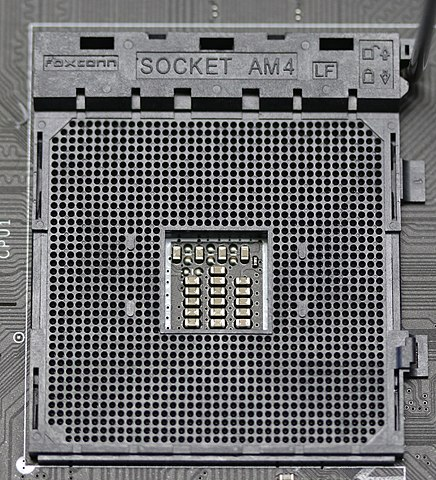
\includegraphics[width=\linewidth]{socket_pga.jpg}
        \end{minipage}
        \vspace{10pt}

        \begin{minipage}{0.6\linewidth}
            \setlength{\parskip}{1.2em}
            \item \textbf{LGA}: De \textit{land grid array}, o matriz de contactos en rejilla. En este caso el procesador \textbf{no cuenta} con pines, sino que es una matriz de contactos chapados en oro. Esta rejilla de contactos hacen contacto con el zócalo de la placa base que es la que cuenta con unos pequeños pines flexibles.
        \end{minipage}
        \hfill
        \begin{minipage}{0.3\linewidth}
            \hfill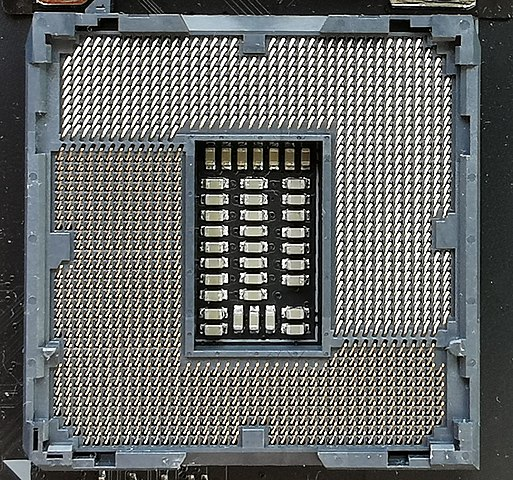
\includegraphics[width=\linewidth]{socket_lga.jpg}
        \end{minipage}
        \vspace{15pt}

        \item \textbf{BGA}: De \textit{ball grid array}, o matriz de rejilla de bolas. El procesador cuenta con unas bolas de estaño que al calentarse se sueldan a la placa base. Hoy en día se utiliza en componentes de tamaño reducido, como en móviles, los chips de memoria en los módulos de RAM, ...
    \end{itemize}

    \item \textbf{Conectores de alimentación}: La placa base tendrá distintos conectores provenientes de la fuente de alimentación con diferentes voltajes, para así proveer de alimentación a los componentes conectados a ella.

    \item \textbf{Ranuras de memoria RAM}: Hoy en día es habitual contar con varias ranuras donde conectar las memoria RAM. Más adelante hablaremos en profundidad sobre la memoria RAM.

    \item \textbf{Chipset}: Es un conjunto de chips, o circuitos electrónicos, que gestionan la comunicación entre los distintos componentes que forman el ordenador, y que están conectados en la placa base. Hoy en día se suelen dividir en dos partes:
    \begin{itemize}
        \item \textbf{Northbridge}: O puente norte. Controla el tráfico de los componentes que trabajan a más alta frecuencia. Comunica el microprocesador, la memoria RAM y la GPU (la ranura PCI express).
        \item \textbf{Southbridge}: O puente sur, comunica los periféricos, los dispositivos de almacenamiento, puertos de entrada/salida como USB, ethernet, ...
    \end{itemize}

    \item \textbf{Ranuras de expansión}: Vamos a identificar estas ranuras como las más modernas  \textbf{PCIexpress}. Son un bus de comunicación de datos de alta velocidad que es usado principalmente para conectar tarjetas gráficas.

    Es cierto que se pueden conectar otro tipo de tarjetas de expansión, como capturadoras de vídeo, tarjetas de red, controladoras RAID, ...

    Hoy en día existen conectores (\textbf{M.2}) donde poder conectar discos duros que tienen un tipo de conector especial.

    \item \textbf{Otros conectores de entrada/salida}: En la placa base existen otros muchos conectores de entrada y salida, que cumplirán distintas funciones dependiendo del tipo de conector, función y/o protocolo de comunicación que utilicen.

    Algunos de estos conectores tendrán conector exterior (al que se podrá conectar directamente el dispositivo), mientras que otros necesitarán de un adaptador (como sucede hoy día con conectores extra USB o el conector “serie”). Algunos ejemplos son:
    \begin{itemize}
        \item \textbf{USB}: Donde poder conectar distintos dispositivos como teclados, ratón, pendrives, mandos de juegos, impresoras, ... El USB (\textbf{Universal Serial Bus}) es un estándar de comunicación de periféricos hoy día. En las placas actuales también hay conectores de tipo \textbf{USB-C}.

        \item Conectores de \textbf{pantalla} como \textbf{VGA}, \textbf{HDMI} o \textbf{DisplayPort}. Dependiendo de lo moderna que sea la placa base, contará con uno o varios de estos conectores.

        \item \textbf{Red}: Hoy día el conector RJ45 es el estándar, que dependiendo de la versión ethernet, nos dará al menos 1Gbit de transmisión. Dependiendo del modelo de placa base también puede tener conectores para realizar conexiones a redes inalámbricas.

        \item \textbf{Audio}: Tanto de entrada como de salida. Normalmente se hace uso de conectores de tipo \textbf{jack}, pero también puede haber conectores de salida digital.

        \item \textbf{Pila}: Las placa base cuentan con una pila para mantener la alimentación para guardar la información de la RAM-CMOS, que es una pequeña memoria que usa la BIOS durante el arranque del sistema.

        \item \textbf{Conectores para ventiladores}: Para regular la temperatura del microprocesador y del interior de la caja, la placa tiene varios conectores que se conectarán a distintos ventiladores que se regularán en intensidad.

        \item \textbf{Otros conectores}: Existen otros conectores para otros puertos que hoy en día no se usan tanto (serie, paralelo, ...) y también los conectores para encender el ordenador, realizar el reset, comprobar el funcionamiento del disco...
    \end{itemize}

\end{itemize}

A continuación un diagrama simplificado de una placa base. Fuente: \href{https://es.wikipedia.org/wiki/Placa_base}{Wikipedia}.
\vspace{-10pt}
\begin{center}
    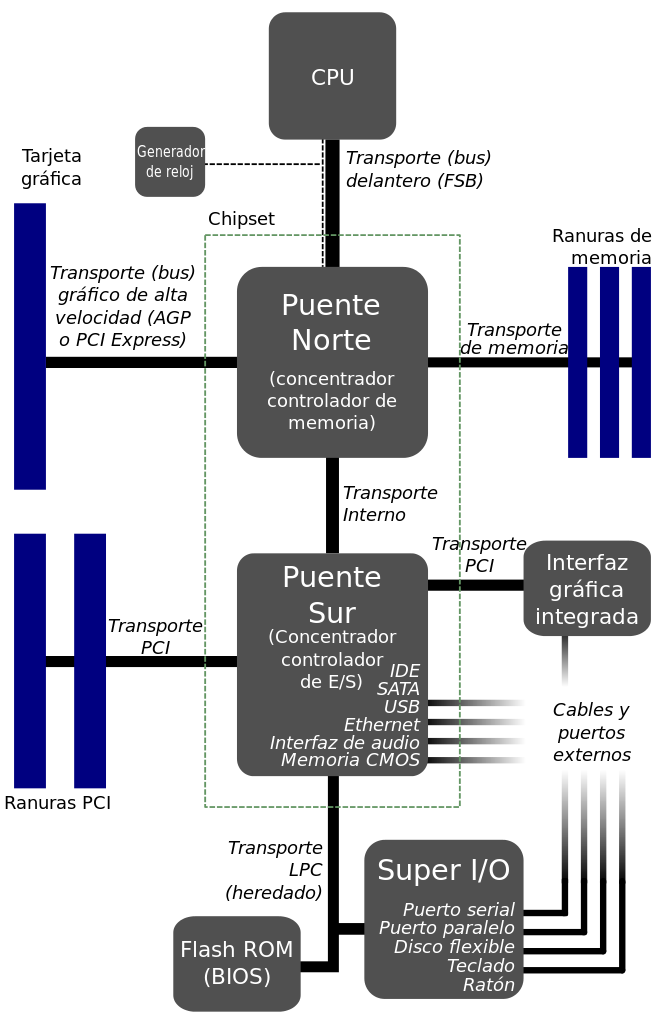
\includegraphics[width=0.56\linewidth]{placa_base_chipset.png}
\end{center}


\subsubsection{Ejemplo de placa base}

A continuación se van a diferenciar los componentes vistos anteriormente en una placa base real, utilizada para crear un equipo de escritorio moderno:

\begin{center}
    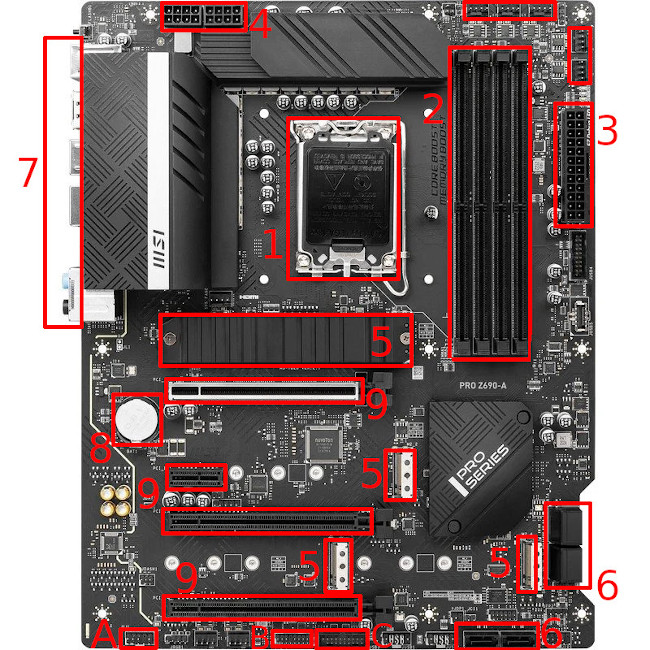
\includegraphics[width=\linewidth]{placa_base.jpg}
    \captionof{figure}{Placa Base MSI PRO Z690-A.  \href{https://download.msi.com/archive/mnu_exe/mb/M7D25v2.0.pdf}{Manual}}
\end{center}

\begin{enumerate}
    \item Zócalo (socket) del procesador.
    \item Ranuras para la memoria RAM.
    \item ATX de alimentación.
    \item Conectores de alimentación extra necesarios por la CPU.
    \item M.2 para discos duros.
    \item SATA para discos duros.
    \item Conectores exteriores (se verán a continuación)
    \item Pila.
    \item Ranuras PCIexpress de distintas velocidades.
    \item[A.] Audio
    \item[B.] Conectores frontales.
    \item[C.] USB 3.0
\end{enumerate}

Los conectores exteriores de esta placa tienen el siguiente aspecto:
\begin{center}
    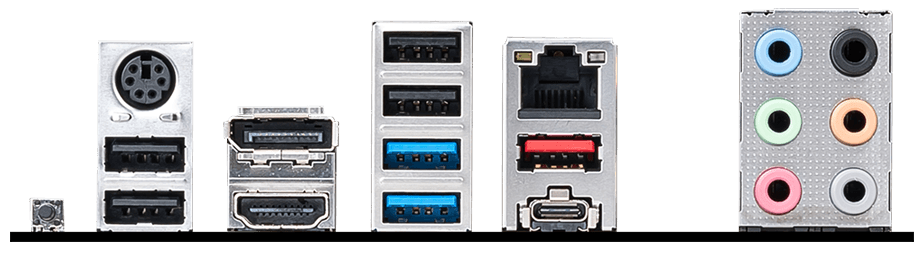
\includegraphics[width=\linewidth]{placa_base_frontal.png}
    \captionof{figure}{Placa Base MSI PRO Z690-A.  \href{https://download.msi.com/archive/mnu_exe/mb/M7D25v2.0.pdf}{Manual}}
\end{center}

De izquierda a derecha, y de arriba abajo:
\begin{itemize}
    \item Pulsador para actualizar la BIOS.
    \item Conector PS2 y USB para actualizar la BIOS.
    \item DisplayPort y HDMI
    \item Usb 2.0 y 3.2
    \item Conector LAN, USB y USB-C
    \item Conectores de audio
\end{itemize}


\subsection{BIOS/UEFI}
La BIOS/UEFI es un interfaz de firmware que está incorporado en un chip en la placa base.

La función principal es la de iniciar el ordenador, realizar una comprobación del hardware del sistema  y se encarga de arrancar el gestor de arranque.

Se ha unificado en esta sección BIOS y UEFI ya que cumplen de manera similar la misma función, pero la segunda es una evolución de la primera.

\subsubsection{BIOS}

El sistema básico de entrada-salida (del inglés \textit{Basic Input/Output System}, o BIOS) lo creó IBM para sus ordenadores “\textbf{Personal Computer}”. Posteriormente se obtuvo por ingeniería inversa las funciones que realizaba tratando de buscar equipos  que fueran compatibles (denominados “PC-compatible”) y de esta manera convirtiéndose en un estándar de facto.

\begin{center}
    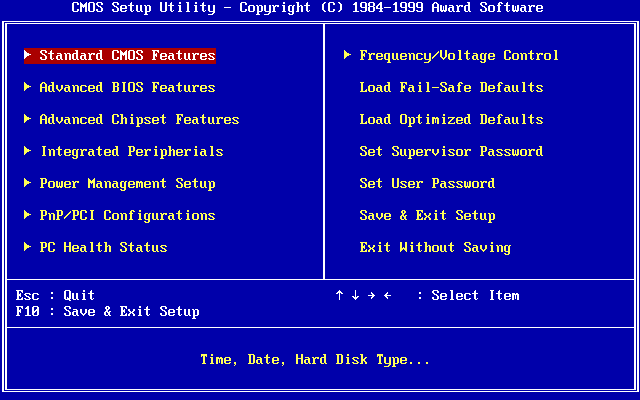
\includegraphics[width=0.7\linewidth]{bios.png}
    \captionof{figure}{Interfaz BIOS. Fuente \href{https://en.wikipedia.org/wiki/BIOS\#/media/File:Award_BIOS_setup_utility.png}{Wikipedia}}
\end{center}

A través de este interfaz se podían configurar algunos aspectos del hardware como las interrupciones de teclado que utilizaban los sistemas operativos antiguos (como MS-DOS), direcciones, el orden del sistema de arranque, ...


\subsubsection{UEFI}
La \textit{\textbf{Unified Extensible Firmware Interface}} (UEFI o «interfaz unificada de firmware extensible») es una especificación pública que define un interfaz entre el sistema operativo y el firmware de la plataforma.


\begin{center}
    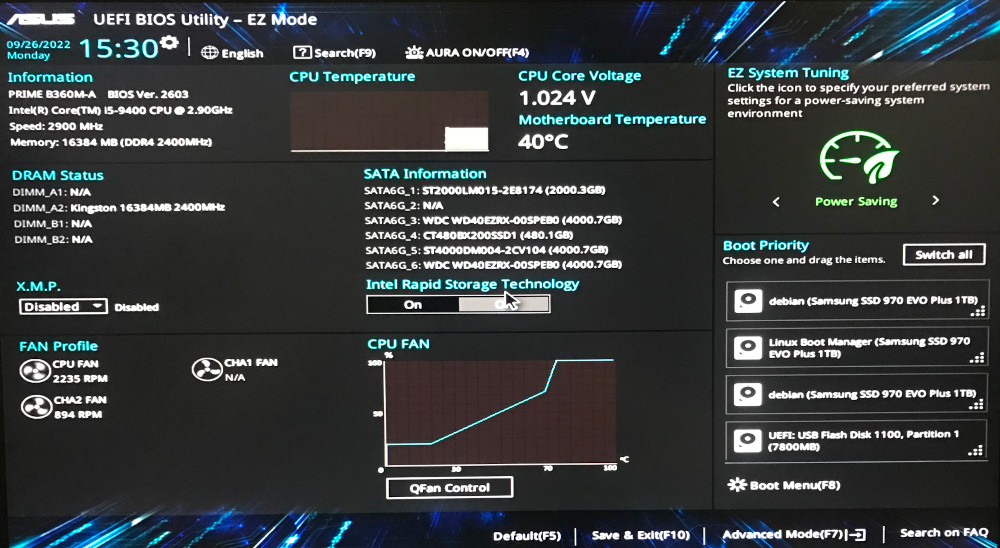
\includegraphics[width=0.7\linewidth]{uefi.jpg}
\end{center}

Se puede considerar una evolución de la BIOS  que tiene las siguientes características:

\begin{itemize}
    \item Permite arrancar desde particiones de más de 2TB.
    \item Diseño modular y extensible.
    \item Retrocompatible con BIOS.
    \item Interfaz gráfica más amigable con el usuario.
\end{itemize}



%\subsection{Procesador}



%
%\subsection{Placa base}
%
%\subsection{Memoria}
%
%
%
%
%\section{Arranque de un ordenador}
%
%\section{Periféricos}
%
%\section{Puertos de conexión}